\documentclass[conference]{IEEEtran}
\usepackage[top=3cm, bottom=2cm, left=2cm, right=2cm, columnsep=20pt]{geometry}
\usepackage{pdfpages}
\usepackage{graphicx}
\usepackage{etoolbox}
\apptocmd{\sloppy}{\hbadness 10000\relax}{}{}
% \usepackage[numbers]{natbib}
\usepackage[T1]{fontenc}
\usepackage{ragged2e}
\usepackage[french]{babel}
\usepackage{listings}
\usepackage{color}
\usepackage{soul}
\usepackage[utf8]{inputenc}
\usepackage[export]{adjustbox}
\usepackage{caption}
\usepackage{mathrsfs, amsmath}
\usepackage{amssymb}
\usepackage{float}
\usepackage{csquotes}
\usepackage{fancyhdr}
\usepackage{wallpaper}
\usepackage{siunitx}
\usepackage[indent]{parskip}
\usepackage{textcomp}
\usepackage{gensymb}
\usepackage{multirow}
\usepackage[hidelinks]{hyperref}
\usepackage{abstract}
\usepackage{subcaption}
\usepackage{tabularx}
\usepackage{biblatex}
\addbibresource{bibliographie.bib}

% \renewcommand{\abstractnamefont}{\normalfont\bfseries}
% \renewcommand{\abstracttextfont}{\normalfont\itshape}
\usepackage{titlesec}
% \titleformat{\section}{\large\bfseries}{\thesection}{1em}{}
% \titleformat{\subsection}{\normalsize\bfseries}{\thesubsection}{1em}{}
% \titleformat{\subsubsection}{\normalsize\bfseries}{\thesubsubsection}{1em}{}

\usepackage{xcolor}
\definecolor{codegreen}{rgb}{0,0.6,0}
\definecolor{codegray}{rgb}{0.5,0.5,0.5}
\definecolor{codepurple}{rgb}{0.58,0,0.82}
\definecolor{backcolour}{rgb}{0.95,0.95,0.92}
\lstdefinestyle{mystyle}{
    backgroundcolor=\color{backcolour},   
    commentstyle=\color{codegreen},
    keywordstyle=\color{magenta},
    numberstyle=\tiny\color{codegray},
    stringstyle=\color{codepurple},
    basicstyle=\ttfamily\footnotesize,
    breakatwhitespace=false,         
    breaklines=true,                 
    captionpos=b,                    
    keepspaces=true,                 
    numbers=left,                    
    numbersep=5pt,                  
    showspaces=false,                
    showstringspaces=false,
    showtabs=false,                  
    tabsize=2
}
\lstset{style=mystyle}

\usepackage[most]{tcolorbox}
\newtcolorbox{note}[1][]{
  enhanced jigsaw,
  borderline west={2pt}{0pt}{black},
  sharp corners,
  boxrule=0pt, 
  fonttitle={\large\bfseries},
  coltitle={black},
  title={Note:\ },
  attach title to upper,
  #1
}

\pagestyle{plain}
%----------------------------------------------------

\setlength{\parindent}{0pt}
\DeclareCaptionLabelFormat{mycaptionlabel}{#1 #2}
\captionsetup[figure]{labelsep=colon}
\captionsetup{labelformat=mycaptionlabel}
\captionsetup[figure]{name={Figure }}
\captionsetup[table]{name=Tableau}
\newcolumntype{Y}[1]{>{\Centering\hspace{0pt}\hsize=#1\hsize}X}
\newcommand{\inlinecode}{\normalfont\texttt}
\usepackage{enumitem}
\setlist[itemize]{label=\textbullet}

\begin{document}

%----------------------------------------------------
\title{Microscope\\
\large Travail préparatoire \\
PHS3910 -- Techniques expérimentales et instrumentation\\ 
Équipe L3}

\author{\IEEEauthorblockN{Émile Guertin-Picard}
\IEEEauthorblockA{2208363}
\and
\IEEEauthorblockN{Maxime Rouillon}
\IEEEauthorblockA{2213291}
\and
\IEEEauthorblockN{Marie-Lou Dessureault}
\IEEEauthorblockA{2211129}
\and
\IEEEauthorblockN{Philippine Beaubois}
\IEEEauthorblockA{2211153}
}

\maketitle

\textit{\textbf{Résumé} -- yap yap}

\section{Introduction}


\textcolor{red}{yap yap}


\section{Méthodes \label{methodes}}
Le système optique utilisé pour la conception du microscope est illustré de manière simplifiée
dans la figure \ref{sys} ci-dessous.
\begin{figure}[H]
  \centering
  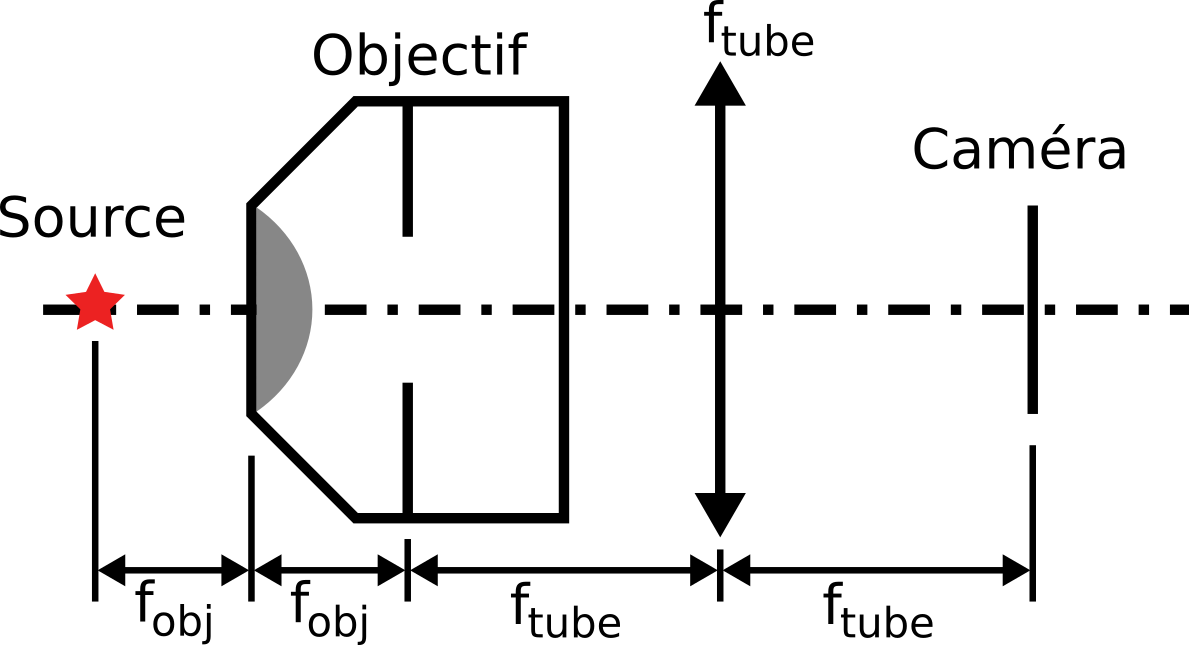
\includegraphics[scale=2.3]{systeme.png}
  \caption{Système optique simplifié du microscope.}
  \label{sys}
\end{figure}
Afin de simuler les observations et les analyses qui seront faites avec le microscope,
une modélisation du mouvement d'une particule a premièrement été effectué sur un scripte Python.
Pour les fins du projet, il a été décidé que de simuler une seule particule serait suffisant pour
évaluer les paramètres à optimiser. En guise d'équivalence de la magnification réelle du microscope, 
une taille de pixel effective $P$ a eu besoin d'être posée. Le calcul de cette taille $P$ est obtenue à partir du grossissement $M$ de l'objectif ainsi qu'avec la
focale de la lentille de tube $f_{tube}$. Le grossissement est défini tel que :

\begin{equation}
  M = \frac{f_{tube}}{f_{obj}},
\end{equation}

où $f_{obj}$ est la longueur focale de la lentille objectif. Le grossissement $M$ connu des lentilles suit
un standard de la \textit{Royal Microscopical Society} (RMS) qui pose $f_{tube}$ à 160 mm
\textcolor{red}{source A}. Ainsi, pour avoir le grossissement réel $M_{r}$, il faut convertir avec la 
formule suivante :

% Source A : https://www.microscopyu.com/microscopy-basics/infinity-optical-systems

\begin{equation}
  f_{1}= \frac{160 \text{ mm} }{M} \Rightarrow M_{r} = \frac{f_{obj}M}{160 \text{ mm} }.
\end{equation}

La taille réelle d'un pixel de caméra $p_r$, d'une valeur de 3.45 µm pour la caméra Zelux CS165MU
mise à disposition pour ce contrat \textcolor{red}{source B}, peut être convertie en taille effective
avec le grossissement réel :

\begin{equation}\label{pixel}
  P = \frac{p_{r}}{M_{r}} = \frac{p_{r}\;160 \text{ mm}}{f_{obj}M}.
\end{equation}



Pour créer un environnement plus fidèle à la réalité, un fond de bruit
a été rajouté, où les photons émis suivent une distribution de Poisson avec \textit{np.random.poisson}. En raison de la diffraction 
causée par le système optique, la particule a due être simulée
telle qu'elle serait perçue par la caméra dans le montage réel. En fonction des composantes optiques utilisées,
la PSF (\textit{Point Spread Function}) de la particule sur le capteur est décrite par:
\begin{equation}
  PSF(r)=\left(\frac{2J_1(\frac{2\pi \text{NA}r}{\lambda})}{\frac{2\pi \text{NA}r}{\lambda}}\right)^2,
\end{equation}
où NA est l'ouverture numérique de l'objectif, $\lambda$ est la longueur d'onde de la lumière passant à travers
le microscope et r est la distance radiale par rapport à la position de l'émetteur \textcolor{red}{source procédurier}. Ici, $J_1$
est une fonction de Bessel. L'émission des photons dans le temps s'effectue selon une distribution de Poisson:
\begin{equation}
  P(X=k)=\frac{\lambda^k e^{-\lambda}}{k!},
\end{equation}
où $k$ est le nombre d'évènements et $\lambda$ est le nombre moyen d'évènements
survenus au cours d'un intervalle de temps $\Delta t$ (le temps d'acquisition). Numériquement, ceci correspond à effectuer un nombre de simulations
d'émission choisi avec \textit{np.random.poisson} et un $\lambda$ arbitraire. La position de chaque photon
émis durant la simulation est déterminée à l'aide de la distribution de probabilité imposée par la fonction d'étalement 
de la particule ($PSF$).

\textcolor{red}{mouvement brownien!!!!}

Après avoir simulé le mouvement d'une particule, l'analyse a pu être effectuée en utilisant une procédure similaire
à celle qui sera utilisée pour le système réel. Pour chaque image capturée lors de l'acquisition (définie par un temps d'acquisition $\Delta t$), un \textit{fit}
d'une gaussienne 2D a été effectuée avec la librairie \textit{lmfit}. La fonction gaussienne 2D est définie par:
\begin{equation}
  f(x,y)=A\cdot exp\left(-\left[\frac{(x-x_0)^2}{2\sigma_x^2}+\frac{(y-y_0)^2}{2\sigma_y^2}\right]\right)+B.
\end{equation}
À partir de la fonction obtenue, les moyennes en $x$ et en $y$ ($x_0,y_0$) de la gaussienne sont obtenus
pour déterminer la position de la particule à cet instant. En effectuant ce processus pour chaque image de l'acquisition,
on a pu obtenir le déplacement général de la particule pour un certain lapse de temps.

Afin de déterminer quels objectifs de microscope considérer pour le produit final, la définition
de la résolution est nécessaire pour la vérification du théorème d'échantillonage de Nyquist. Soit $d$,
la limite de diffraction pour une source ponctuelle au travers d'une ouverture \textcolor{red}{source video}:
\begin{equation}
  d = \frac{\lambda}{2 \text{NA}},
\end{equation}

où $\lambda$ est la longueur d'onde éclairant l'échantillon observé et NA est l'ouverture numérique de
l'objectif. Cette limite de diffraction est la résolution du système. Ainsi, selon le théorème
de Nyquist, la taille effective d'un pixel de la caméra $P$ dans le plan de l'objet observé doit respecter :

\begin{equation}\label{nyquist}
  P \leq \frac{d}{2} = \frac{\lambda}{4 \text{NA} }.
\end{equation}


Ainsi, pour un système avec $f_{obj}$ et $M$ connus (voir équation \ref{pixel}), il est possible de déterminer si le théorème 
(\ref{nyquist}) est respecté pour une longueur d'onde donnée. Cela a permis de déterminer quelles 
combinaisons de lentille tube, d'objectif de microscope et de source de lumière qui ne sont pas 
sujettes au phénomène d'\textit{aliasing}, conséquence du non respect de Nyquist où l'information
réelle sur l'image est perdue.

% source B : https://www.thorlabs.com/thorproduct.cfm?partnumber=CS165MU

\section{Résultats \label{resultats}}



\section{Discussion}

\textcolor{red}{quel combo a la meilleure resolution $d$ avec le moins d'incertitude}

%\printbibliography

\clearpage

\section{Annexes}

\subsection{Preuve de correction par Antidote}

\clearpage


\end{document}
